\section{Qualitative analysis}


We selected 30 brainstorming runs (5 randomly from each condition). The primary author applied an open coding strategy, identifying classes of ideas within runs that hold common characteristics. For each class that was observed across multiple participants, we infer the existence of a \emph{strategy}: a plan or rule that aids in generating ideas. We describe the observed strategies in detail below.
We describe the distribution of these strategies across runs and comment on variability between participants.

\subsection{Strategies}

A \emph{strategy} is a plan or rule, that is used by a participant to generate brainstorming responses.
We identified 3 \emph{orthogonal} strategy categories - each category of strategies can be employed by a participant with or without any of the other categories.
The first, \emph{problem scoping}, is a process in which a participant chooses a limited implication or component of the problem and provides multiple specific solutions.
The second category expands on the \emph{riffing} phenomenon introduced earlier, identifying 4 different types of riffing.
%Finally, the \emph{humour} strategy emphasizes generating ideas that are amusing rather than practical.
Finally, the \emph{partial solution} strategy entails creating an idea that requires further idea generation to solve the problem.

\subsubsection{Problem scoping}

Under the problem scoping strategy, the original problem is transformed to a new problem of reduced scope.
Many transformations of the MP3 problem are possible, for example: brainstorm uses for \emph{an audio output device}; brainstorm uses for a small box-shaped object; brainstorm uses for \emph{a hard drive}; and so on. The participant chooses a problem transformation and generates solutions, each of which is also a solution to the original problem. For example (PXXX):

\begin{itemize}
    \item have them as a resource on public transportation -- people must supply their own headphones
    \item use them in museums to give information on various installations
    \item have cities install them in tourist areas, so people can listen about where they are
\end{itemize}

The participant's responses satisfy the transformed question "brainstorm uses for an audio output device". Resulting ideas no not rely on other aspects of the problem.

We distinguish between two types of problem scoping. \emph{Inward scoping} transformations reduce scope by limiting consideration to a single detail of the problem. The previous responses, which focus on audio output, are an example of inward scoping.

\emph{Outward scoping} transformations reduce complexity by stripping all meaningful details. For example (PXXX):

\begin{itemize}
    \item doorstop
    \item use in abstract art
\end{itemize}

These solutions could be applied to a wide body of problems unrelated to the original, such as "brainstorm uses for a broom".
In contrast, inward scoping solutions are applicable to the transformed problem and the original problem, but not many others. Thus, a useful rule for distinguishing the types of scoping is to consider whether the \emph{set of problems solved by the solutions} is small, or large.

Some responses employ no scoping whatsoever. These responses utilize the device exactly as it was intended, as a portable MP3 player. For example, "get it fixed and give it to a needy kid" (PXXX).

\subsubsection{Riffing}

The second category of strategies is \emph{riffing}.
We found riffing manifested itself many ways, and identified four distinct riffing strategies used by participants: generalization riffing, repeat riffing, hold riffing, and continuation riffing. 

\emph{Generalization riffing} occurs when a participant generates two or more ideas and one is a generalization of the other. For example, two consecutive ideas given by PXXX:

\begin{itemize}
    \item brick
    \item building material
\end{itemize}

Another type of riffing is \emph{repeat riffing}. Under this strategy, a participant produces multiple responses with only slight differences between them, such that the group of ideas could be easily summarized as one idea without significant loss of information. For example (PXXX):

\begin{itemize}
    \item extract usage data
    \item extract texts
    \item extract gps data
\end{itemize}

In this case, all three ideas could be summarized with "extract the data on the device".

\emph{Hold riffing} is a strategy in which participants hold at least one element of a previous response constant when generating a new response, such that a new idea is formed. For example (PXXX):

\begin{itemize}
    \item Jukebox music selector in bars
    \item Commercials in bar bathrooms 
    \item Tapper handles for beer 
\end{itemize}

In this example, the setting of the application is held constant across riffs: a bar.

Another realization of hold riffing holds language term constant between unrelated ideas. For example (PXXX):

\begin{itemize}
    \item We could use the hard-drives inside for different electronics.
    \item We could use them in place of rocks (to throw at things, to use in pavement.)
\end{itemize}

\emph{Continuation riffing} is the strategy of creating another idea that relies on the implications or consequences of a previous idea. The new idea cannot be understood without the context of the previous. For example (PXXX):

\begin{itemize}
    \item I suppose you could just grind them down into a sand
    \item You could take the sand... and put it in an hourglass
\end{itemize}

\paragraph{Spatial separation}

The strategies above describe techniques for taking one idea and transforming it into another. In this section, we describe patterns of \emph{where} participants implemented these strategies.

The most natural separation between a riffed idea and its source is none - the riffed idea directly follows the source. We call this \emph{linear riffing}.
\emph{Reach backs} entail riffing on an idea that occurred further back in the run than the previous response. 

Finally, some participants \emph{pair} their riffs. Paired riffing is a special case on linear riffing in which only a single riffed idea is produced, and no further riffs are produced on that source for the remainder of the run. For example, paired repeat riffing from PXXX:

\begin{itemize}
\item cut up and use to decorate shoes
\item cut up and use to decorate vase
\end{itemize}


\subsubsection{Partial solutions}

Under this category of strategies, responses provide some elements of a solution to the problem, but further idea generation is required to implement the solution. The following ideas (PXXX) are all examples of partial solutions:

\begin{itemize}
    \item use old parts to make a new device
    \item old parts can use to make something
    \item create a new device
\end{itemize}

In these responses, there is a clear recommendation that we recycle components of the MP3 player to produce new electronics, but it is unclear what we would make or how we would use the parts. 

There are four sub-strategies of partial solutions: problem scoping without solution, goal without plan, plan without goal, and passing the problem. 
In some responses, an end goal has been established, but any implementation of the goal requires further idea generation. We call this strategy \emph{goal without plan}. The above responses are examples of the goal without plan strategy.
The goal of creating a new electronic device is given, but it is not clear what will be created or how the materials will be re-used.

The inverse of this strategy is \emph{plan without goal}, as demonstrated in these responses (also from PXXX):
\begin{itemize}
    \item melt down old parts
    \item see what old parts are usable
\end{itemize}
In this case, the operations of melting down the device or checking for working parts can be performed, but don't provide any obvious benefit.

Above, we described the problem scoping strategy. Some participants performed \emph{problem scoping without solution}, in which problem scoping is the only component of the response.
For example, one of PXXX's responses to the MP3 player problem was to "Remove glass screen to make something". In this case, the participant has provided a scoping of the problem (focus on the glass component) but has not actually provided a solution to the scoped problem.

Responses that do not have an explicit goal or plan may nonetheless imply one. For example, "throw it in the ocean" (PXXX) has the implied goal of disposing of the broken device. In these cases, responses do not employ a partial solution strategy.

Finally, responses in the \emph{pass the problem} strategy relocate the need for idea generation to a third party. These responses from PXXX provide an example:

\begin{itemize}
    \item give to non-profit that can benefit
    \item give to an organization that has the knowledge to use these devices
\end{itemize}

These solve the original problem, but simultaneously re-open the problem under slightly changed conditions. In this case, a third party must determine what to do with broken MP3 players.

\subsection{Strategy use}

In this section, we DESCRIBE how strategies were employed by participants. The primary author again coded 30 randomly selected runs (5 from each condition, 1150 instances total) for the strategies identified above. Note that examples of riffing identified in this section are distinct from the category tree identification of riffing described in the method section above. The prevalence of each strategy as a function of total number of instances is given in Table TAB, and a comparative plot in Figure FIG.

\begin{table}
    \begin{tabular}{r | l l}
        \textbf{strategy} & \textbf{\# instances} & \textbf{\% of instances} \\
        inward scoping & 267 & 23.2 \\
        outward scoping & 828 & 72 \\
        no scoping & 55 & 4.8 \\
        \hline \hline
        hold riffing & 278 & 24.2 \\
        continuation riffing & 3 & 0.3 \\
        repeat riffing & 119 & 10.3 \\
        generalization riffing & 48 & 4.2 \\
        \hline
        any riffing & 448 & 39.0 \\
        pair & 108 & 9.4 \\
        reach back & 129 & 11.2 \\
        \hline \hline
        scoping without solution & 3 & 0.3 \\
        passing the problem & 69 & 6 \\
        plan without goal & 58 & 5.0 \\
        goal without plan & 58 & 5.0 \\ 
        \hline
        any partial solution & 188 & 16.3 \\
    \end{tabular}
\end{table}

\begin{figure}[h!]
    \centering
    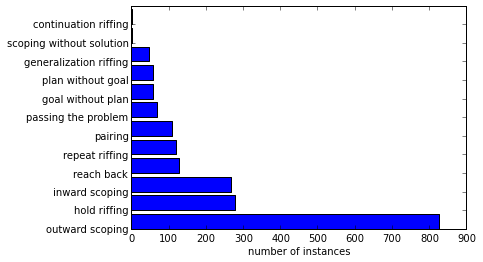
\includegraphics[width=0.9\columnwidth]{strategy_counts}
    \caption{presence of strategies}
    \label{fig:strategy_counts}
\end{figure}

Outward scoping is by far the most commons strategy, occurring in 72\% of instances. Riffing is also very common, with 40\% of instances employing some form of riffing. Riffs are most often consecutive (linear riffing), and hold riffing is the most common type.

Partial solutions are fairly uncommon (16.3\%), and most often involve passing the problem (6\%). Continuation riffing and scoping without solution are the least common strategies, each with only 3 instances.

\subsubsection{Strategy location}

We also consider where in a brainstorming run the strategies are more likely to occur. The results are summarized in Table TAB.

\begin{table}
    \begin{tabular}{r | l l l l l l}
        \textbf{strategy} & \textbf{5} & \textbf{10} & \textbf{25} & \textbf{50} & \textbf{75} & \textbf{100} \\
        inward scoping & 2 & 5 & 11 & 23 & 29 & 44 \\
        outward scoping & 3 & 3 & 8.5 & 27.5 & 39.5 & 41 \\
        no scoping & 3 & 5 & 9 & 18 & 22.5 & 20.5 \\
        \hline \hline
        hold riffing & 3 & 8 & 12.5 & 24 & 44.5 & 57.5 \\
        continuation riffing & - & - & 18 & 4 & 27 & - \\
        repeat riffing & 4 & 7 & 2 & 25 & 49.5 & 45 \\
        generalization riffing & 4 & 4 & 11 & 29.5 & 34 & 30 \\
        \hline
        pair & 3.5 & 7.5 & 12.5 & 25.5 & 40 & 33.5 \\
        reach back & 3.5 & 6 & 11 &29.5 & 40 & 47.5 \\
        \hline \hline
        scoping without solution & - & - & - & 13 & - & 53 \\
        passing the problem & 1.5 & - & 14.5 & 40 & 35.5 & 60.5  \\
        plan without goal & - & - & 6 & 18 & 38.5 & 30 \\
        goal without plan & - & 3 & 2 & 15 & 11 & 29 \\ 
    \end{tabular}
    \caption{Median position of strategy in run by condition}
\end{table}

The distributions of strategy occurence across position in run tend towards uniform when there are more than a few examples. The notable exception to this is problem scoping. There are fewer occurences of the inward scoping strategy later in brainstorming runs.

The number of reach-backs increase with position. This may simply be because there are more ideas to draw from for inspiration later in a run.

%\subsubsection{Strategy co-occurrence}

%Of final interest was the question of which strategies occurred together. For each run, a count was taken of the number of occurrences of each strategy, and the Pearson r of these counts was taken for each pairing of strategies to give a rough measure of how the strategies were grouped in runs. Strong correlations (greater than 0.6) are given in Table TAB.

%\begin{table}
%    \begin{tabular}{l l l}
%        \textbf{strategy 1} & \textbf{strategy 2} & \textbf{Pearson r} \\
%        \hline
%        passing the problem & repeat riffing & 0.89 \\
%        hold riffing & outward scoping & 0.85 \\
%        pairing & scoping without solution & 0.64 \\
%        reaching back & hold riffing & 0.64 \\
%        pairing & outward scoping & 0.63 \\
%        reaching back & outward scoping & 0.62 \\
%        plan without goal & hold riffing & 0.61 \\
%    \end{tabular}
%\end{table}

%Passing the problem and repeat riffing were highly correlated (0.89), indicating that responses utilizing pass the problem were likely to be repeated many times to generate more responses. For each of the other correlations, the potential implications less obvious. Further analysis is required to tease out the implications of strategy co-occurrence.

\subsection{Variability of Worker Input}
While we observed that individuals are likely to draw from a common pool of ideas early on in the brainstorming process, there were outliers in the data. For example, one individual in the 75 ideas condition consistently produced some of most original ideas for old MP3 players:

\begin{itemize}
\item With displays - could be attached to a small solar panel (like the USB chargers w/multi attachments, including solar and car, etc.) and all the power could be sent to the screen as a small, portable light, then sent to countries lacking power in rural areas.
\item They could be loaded with coordinates or other info and sealed in containers, then used in ocean current studies - once the container was collected they could be plugged in and read, and the data could be sent to whomever.
\item They could be plugged in at a base camp at the bottom of Everest, and then potential climbers could record their name, loved ones' address, and any last words before attempting the climb. 
\end{itemize}

This individual's responses were responsible for clearly raising the observed uniqueness of ideas in the 75 condition when plotted against the other conditions.
In contrast, other individuals filled their quotas with excessive repeat riffing chains. 

This variability in worker responses prevented us from modeling any potential effects that the number of questions requested might have on individuals' responses. Thus, while it is clear that there is little advantage to requesting 5 or 10 ideas from workers, it is not clear whether it is preferable to request 20, 50, 75, or 100 ideas. We suspect that requesting 50 or 75 is the ``sweet'' spot, but are not able to empirically support that recommendation at this time.


